\section{Wind Cave National Park}

\subsection{Current Grassland Management Goals and Programs}

\subsubsection{Grassland Management Goals}

\paragraph{Diverse ecosystems}
Wind Cave National Park (WICA) is set
within the eastern slope of the Black Hills region of South Dakota.
Because of this, it has an array of ecosystems ranging from montane
woodlands to open grasslands. It is also unique in that it has a teeming
ecosystem underground within the cave that the unit is known for. This
variety in ecosystems and processes requires a diverse set of management
goals. The Foundation Statement voices the desire to maintain wildlife
populations with the acknowledgement of maintaining natural plant
communities.

\paragraph{Water}
Another management goal is groundwater. Pressures from
outside the park are impacting both quality and quantity of groundwater
reaching the park. Interviews revealed that the park staff expect
development and thus pressures to only grow in the future. Overall, they
desire management to focus on how best to maintain the natural state of
the ecosystem.

\subsubsection{Grassland Management Programs}

\paragraph{Wildlife Management Program}
Wildlife management includes the
most pure herd of bison in the NPS system. Many satellite herds of the
WICA herd exist across the MWR. This has spawned the creation of the
Bison Leadership Team which is assessing the status of bison and the
grazing resources it depends on. Reintroductions at WICA include black
footed ferret, bison, elk and pronghorn. Management plans for these
species include an aspect of ecosystem effects.

\paragraph{Invasive Species Management}
Over the last two years, rather
than the EPMT visiting Wind Cave, they have managed invasive species
with their own budgets and staff. The unit was not approved for use of
chemicals until 2011. Without fire and herbicide, invasive species has
expanded across the park. Most impactful invasive species are Canada
thistle, leafy spurge, and horehound. The park has ramped up its
herbicidal efforts in the last few years for these species.

\subsection{Management Plans and Data Available}

\subsubsection{Management Plans}

Along with the Zoning Management Plan, there have been several other
strategies written from 2008-2018. Although, a vegetation management
plan, fire management plan and many wildlife management plans fall
outside of the last ten years. Although these directives are in all
likelihood still followed, operating on information that is over 10
years out of date is keeping the unit from most skillfully managing the
landscape. A full list of management documents published from 2008- 2018
is displayed in Table~\ref{tab:WICAmandocs}.

According to the foundation document for the park, with a draft document
written in 2011, the desired conditions for vegetation are to maintain
healthy plant communities and to further research endemic flora. At the
time this document was written, 20-25\% of the landscape was ponderosa
pine ecosystem type and 75-80\% was prairie. This showcases the
uniqueness of this area as a ``mixing zone'' of ecosystem components.

\begin{table}[h]
	\centering
\caption[WICA Management documents]
	{Management documents for WICA published from 2008-2018}
\label{tab:WICAmandocs}
\begin{tabular}{lc}
	\toprule
	Title & Year\tabularnewline
	\midrule
Integrated Pest Management Plan & 2010* \tabularnewline
Foundation Statement & 2011* \tabularnewline
Invasive Species Action Plans & 2010-2018 \tabularnewline
Elk Management Plan & 2009 \tabularnewline
Natural Resource Condition Assessment & 2011 \tabularnewline
Long Range Interpretive Plan & 2012 \tabularnewline
Zoning Management Plan & 2015 \tabularnewline
\bottomrule
\end{tabular}
\end{table}

Interview responses expressed that these plans are written by species and then integrated to manage ecosystem wide. 
Ecosystem management goals have not been laid out within the last ten years. 
A comprehensive management plan with current management plans would benefit WICA. 
This would make the integration of single resource management plans seamless.

\subsubsection{Data Available}

WICA has a significant amount of ecosystem data. 
It is fairly spread among resources as well. 
Staff at WICA, compared to other parks is fairly specialized giving focus to data collection for different resources at the park. 
WICA is the only unit with a designated, permanent vegetation specialist on staff.

%\storeareas\normalsetting
\KOMAoption{paper}{landscape}
\areaset{1.5\textwidth}{.6\textheight}
\recalctypearea
\pagestyle{plain}
\setlength\LTcapwidth{1.5\textwidth} 
\setlength\LTleft{0pt}           
\begin{longtable}[l]{@{}p{5cm}p{2cm}p{3cm}p{4cm}p{3cm}p{4cm}p{3cm}@{}}
	\caption[WICA data]
	{Selected data collected in WICA, 2008-2018.} 
	\label{tab:WICAdata} \\
	\toprule
	Data title & Data type & Spatial extent & Frequency & Duration & Collecting agency & Format located \tabularnewline
	\midrule
	\endfirsthead 
	\caption* {\textbf{Table \ref{tab:WICAdata}}, \emph{continued.}} \\
\toprule
Title of Data & Type of Data & Spatial Extent & Frequency of Collection & Duration of Collection & Agency Collecting Data & Format Located \tabularnewline
\midrule
\endhead
Develop Forage Production and Allocation Model for WICA & Vegetation &
cages across the park and using the park GIS to get the rest of the data
other than production & once & 2008 & University of Missouri- Columbia/
NPS & site network\tabularnewline
AUM Range Stocking Rate & Wildlife/ Vegetation & site wide & range
assessments each year & 2001-2009 & NPS/ NRCS & site
network\tabularnewline
Park rare plant survey/monitoring & vegetation & site wide & ~ &
2004-2008 & NPS & site network\tabularnewline
Scotch Thistle locations & Vegetation & sitewide & ~ & 2000-2008 & NPS &
site network\tabularnewline
Forage Management WICA & Vegetation & sitewide & range assessments each
year & 2001-2008 & NPS & site network\tabularnewline
Pronghorn Survey & Wildlife & sitewide & this count was in 2010 & 2010 &
NPS & site network\tabularnewline
Fuel Sampling History & Vegetation & sitewide & this was an assessment
of previous data ahead of the begin of the Fire Effects monitoring
through I\&M & 2011 & NGP I\&M & site network\tabularnewline
Reduce highly invasive white horehound impacting prairie dog/
black-footed ferret habitat & Vegetation/ Wildlife & prairie dog towns
across the unit & applications of herbicide in 2009-2011 & 2009-2012 &
NPS & site network PMIS\tabularnewline
Water Resources of WICA & Water & parkwide & an overview of water
resources in the unit & 2016 & NPS & site network\tabularnewline
Example of Herbicide application data sheets & Vegetation & specific
sites within the park & each application & 2016 & NPS & on
site\tabularnewline
Bison, Pronghorn and Butterfly Survey & Wildlife & parkwide & once &
2015-2017 & NPS & on site\tabularnewline
Habitat restoration guidelines for highly disturbed natural areas
(prairie dog towns) following invasive weed eradication & Vegetation &
prairie dog towns across the unit & ~ & 2009 & NPS & on
site\tabularnewline
Determine strategies for efficient early detection of invasive plants
after prescribed fire & Vegetation & 215 plots site wide & once each
year (pre-burn and post-burn) & 2010-2012 & USGS, NGPFire & on
site\tabularnewline
Monitoring of Sharp-tailed Grouse Leks in WICA & Wildlife & parkwide &
once in spring & 1999-2011 & NPS & on site\tabularnewline
Monitoring Bird Populations in WICA using point counts and autonomous
recording units & Wildlife & parkwide & once & May-July 2008 & Rocky
Mountain Bird Observatory & on site\tabularnewline
WICA Nightjar Survey & Wildlife & parkwide & 2 survey routes per year &
2009-2017 & NPS & on site\tabularnewline
WICA precipitation & Weather & parkwide & average each month & 1983-2017
& NPS & site network\tabularnewline
Bison Population Numbers & Wildlife & parkwide & yearly numbers &
1996-current & NPS & site network\tabularnewline
Vegetation Projections for WICA with Three Future Climate Scenarios &
Vegetation & parkwide & modeled using already collected data & 2013 &
Oregon State University/ USGS & site network\tabularnewline
Vegetative Reproduction and Bud Bank Dynamicsof the Perennial Grass
Andropogon gerardii in Mixedgrass and Tallgrass Prairie & Vegetation &
parkwide & once & 2010 compared to previously collected data in 2008 &
Kansas State University & site network\tabularnewline
What role does prescribed fire play in managing annual bromes in
northern Great Plains grasslands? & Vegetation & inside edges of
Headquarters east burn unit/ inside edges of Bison Flats burn unit & ~ &
~ & USGS/NPS & on site\tabularnewline
An Adaptive Management Framework to Control Cheatgrass in Norhtern Great
Plains Parks & Vegetation & parks throughout the MWR & ~ & ~ & NPS &
PMIS\tabularnewline
Vegetation Baseline for Casey Addition in WICA & Vegetation & new
addition to WICA & ~ & ~ & NPS & PMIS\tabularnewline
\bottomrule
\end{longtable}
\clearpage
\normalsetting
\pagestyle{fancy} 

\subsection{Disturbance Regime }

\subsubsection{Grazing }

Livestock grazing was common in the area before establishment of WICA in
1903. In 1913, management began of a bison herd. The bison management
plan, written in 2006, discusses the cultural and genetic importance of
the herd while also acknowledging effective use of the range. The focus
of bison management lies on maintaining a viable genetic population. The
park maintains a herd of near 400 animals using over 28,000 acres of
mixed grass prairie and Ponderosa pine forest. Bison at WICA are free to
move about the entire park. The herd at WICA had consistently lower body
weights compared to other parks. This could be attributed to poor forage
quality within the unit or herd changes due to lack of predators or
climate change (Licht, 2016). Elk, mule deer and pronghorn also
contribute to the grazing disturbance at the park.

\subsubsection{Fire }

Wind Cave National Park was the first MWR unit to reinstate prescribed
fire in 1973 following decades of complete suppression (Wienk et al.,
2011). The largest threats to WICA are fuel loads throughout the park
(Interviews, 2018). Fire has not occurred as frequently as it could and
is highly susceptible to a stand replacing fire. In the last ten years
there have been ten prescribed fires with some years seeing no fire.
Minimal use of fire has created a mosaic on the landscape (Fig.~\ref{fig:WICAmosaic}).
The zone management plan treats different areas of the unit in different
ways, either letting them burn or extinguish immediately.

\begin{figure}[]
	\centering
	\begin{subfigure}[t]{0.5\textwidth}
		\centering
		\includegraphics[]{WICA_Fire-mosaic}
		\caption{Mosaic created by prescribed fires.}
		\label{fig:WICAmosaic}
	\end{subfigure}%
	~ 
	\begin{subfigure}[t]{0.5\textwidth}
		\centering
		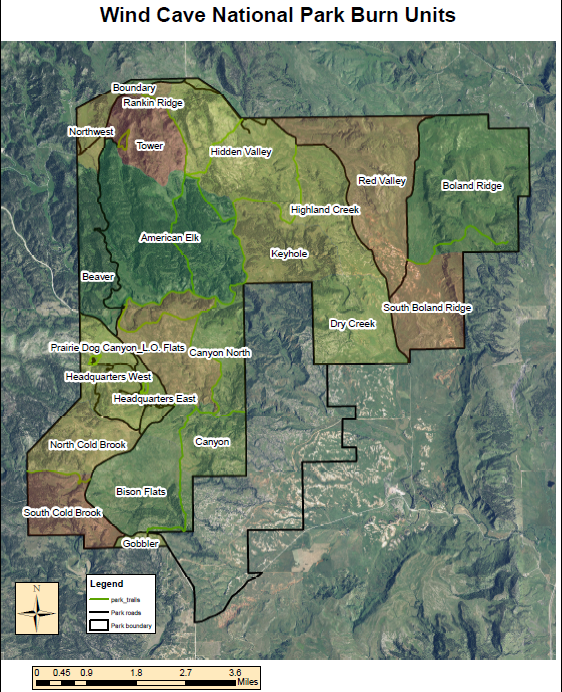
\includegraphics[]{WICA_burn_units}
		\caption{Burn units.}
		\label{fig:WICAunits}
	\end{subfigure}
	\caption[WICA fire maps]{Prescribed fire maps for WICA (Aston \& Davis,
		2016).}
\end{figure}

\subsection{Data gaps and suggested research}

\subsubsection{Data Gaps}

WICA data is substantial in comparison to other units in this study. It
covers many resources and will aid in the development of a coupled
disturbance regime. Understanding the status of resources in the park is
the first step in planning. The effect of disturbance on resources is
the next. Diversity of fuels is an issue at the park. Beneficial data
would be understanding how different ecosystems within the park respond
to varied fire season and varied intensity. The inherent heterogeneity
of the WICA landscape is critical to its character. Imposed disturbance
will be critical in maintaining inherent heterogeneity. For example, in
the last year, a stand replacing fire occurred in the ponderosa pine
ecotone. Diverse fire behavior can have desired effects on the landscape
to remove dangerous fuel loading.

\begin{figure} 
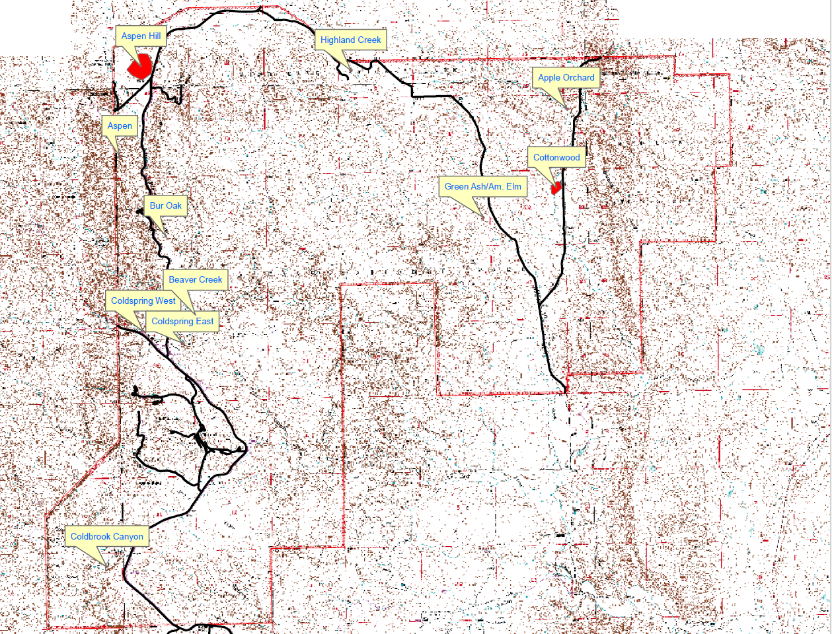
\includegraphics[width=0.8\textwidth]{WICA_exclosures}
\caption{Past exclosure locations within WICA}
\label{fig:WICAexclosures}
\end{figure}

Bison movement in response to fire is also missing. On a fenceless
landscape, bison are free to graze in whatever area they choose. Bison
GPS collars are currently used in BADL, THRO, and WICA. Combining this
with fire data could determine if fire is a beneficial attractant to
bison to move them or disperse them to desired areas of the landscape
naturally. Finally, a vegetation management plan with specific
vegetation goals would aid in the development of a disturbance regime.

\subsubsection{Suggested Research}

There is historical data of exclosure locations in WICA. This makes the
possibility of collecting exclosure clippings to determine vegetation
productivity replicable. Aligning exclosure locations with burn unit
locations is beneficial. A park that protects such vastly different
ecosystems requires a heightened sense of site-specific data.
Productivity data will aid in developing a coupled disturbance regime.
This is needed to determine the amount of disturbance the landscape
would benefit from. The diversity of ecosystems in WICA would benefit
from the following studies:

\begin{itemize}
\item Season of fire effect on vegetation resources
\item Effect of frequent fire on forage quality
\item Response of horehound to patchy fires
\item Bison movement in response to fire
\item Erosion rates in relation to bison occupation
\end{itemize}

\subsection{Management Recommendations}

\subsubsection{Reduce high fuel loads, create disturbance mosaic}

WICA manages the landscape to benefit the ecosystem. Management plans
are written to specific species, but interviews revealed that the
integration of the plans is forefront. Interviews also revealed that the
biggest threat to the unit is wildfire. This may be attributed to recent
events in the park, but is a definite concern nonetheless. The landscape
at WICA requires a varied disturbance regime. One way to achieve this is
through pyro diversity. Fire in the mixed-grass prairie should be
managed differently than fire in the Ponderosa pine forests. WICA
contains a fire prone ecosystem with large fuel loading particularly in
the forested regions of the unit. Prescribed fires may not remove all
wildfire threat from the landscape but will significantly reduce the
likelihood of a stand replacing fire.
